\chapter{MegaManaging, Part II: Direction, Growth, and the Design of an Extraordinary Life}

This talk begins in mid-conversation, but it very quickly resets its own stage. We are asked to look first at a ladder of earnings, then at the person who climbs it, then at the guidance system by which a life is steered, and finally at the discipline by which that life is measured and lived. The arithmetic is simple, but it is not trivial. Rohn uses it to make a stronger claim: the real variable is not merely the market outside us, but the value, discipline, and direction we bring into it. These notes follow that progression closely, preserving the order in which the lecture first surprises, then redirects, and only afterward systematizes.

\section{The Income Ladder and the Marketplace of Value}

Rohn's opening move is numerical and provocative. He asks whether income can be multiplied by \(10\), and he asks the question as though it ought to be taught early. The point of departure is deliberately local and concrete. If somewhere nearby a person can be found earning \(\$50\) an hour, then the first jump is no fantasy. If \(\$500\) an hour can be found, the second jump is no fantasy either. He then drives the ladder higher with public examples of speaking fees and large annual earnings, not because the audience is supposed to imitate generals or presidents, but because the mind needs to be forced out of its inherited ceiling.

The opening arithmetic can be summarized as
\begin{align}
50 \times 10 &= 500,\\
500 \times 10 &= 5000.
\end{align}
If we let \(I_n\) denote the \(n\)-th rung of the earnings ladder, then the lecture's repeated scaling move may be written as
\begin{equation}
I_{n+1}=10I_n.
\end{equation}

\begin{remark}
This recurrence is a note-writer's shorthand. It is faithful to the arithmetic of the talk, but it is not itself spoken in algebraic form.
\end{remark}

Rohn strengthens the ladder with benchmark values that are large enough to block easy dismissal:
\begin{equation}
\text{\$65{,}000/hour}, \qquad \text{\$125{,}000/hour}, \qquad \text{\$36 million/year}.
\end{equation}
These are not offered as a doctrine of celebrity compensation. They are used to establish a simpler proposition: the scale exists. Therefore the real question is not whether the scale exists, but what must change in us for access to it to become possible.

From here the lecture pivots immediately into wish and value. America is described as a place in which one may own as much property as one wants or as little as one chooses; it is ``wish-want country.'' But wish is not left as fantasy. To climb the ladder ``as high as you wish'' is quickly restated as bringing value to the marketplace and becoming valuable to the marketplace. Only after that restatement does Rohn give the principle that changed his life:
\begin{equation}
\text{work on your job} \to \text{make a living}, \qquad
\text{work on yourself} \to \text{make a fortune}.
\end{equation}

He then sharpens the point again: success is not something one mainly pursues. It is something one attracts by becoming attractive. The lecture's own mathematical compression of this is still verbal, but its structure is clear.

\subsection{Question \& Answer}

What, then, is actually being multiplied when income scales so dramatically?

Not the hour. Not the day. Not the calendar. The operative term is the value brought to the marketplace. A compact editorial formula for the lecture's mechanism is
\begin{equation}
I \propto V,
\end{equation}
where \(I\) is income and \(V\) is value to the marketplace.

\begin{remark}
Again, \(I \propto V\) is not a quoted board equation. It is a cautious summary of the spoken logic: multiply your value by \(3\) or \(5\), and income can rise by \(3\), \(5\), or even \(10\).
\end{remark}

\paragraph{Worked example.}
The lecture's rule of thumb can be written as
\begin{align}
V &\mapsto 3V \quad \Rightarrow \quad I \mapsto 3I,\\
V &\mapsto 5V \quad \Rightarrow \quad I \mapsto 5I \text{ or more}.
\end{align}
This is not a theorem of finance. It is the lecture's working causal picture. Growth of income follows growth of usefulness, skill, judgment, and personal attractiveness to the market.

The opening section therefore does not end on money. It ends on personal development. We can have more than we have, Rohn says, because we can become more than we are.

\section{Personal Philosophy as a Guidance System}

Only after the ladder and the attraction principle are established does the lecture begin its formal list of five ideas. The first is personal philosophy. Rohn briefly notes that philosophy is a large subject in its own right---spiritual, economic, social, and more---but then narrows the scope with care. The subject here is not philosophy in the library sense. It is personal philosophy in the navigational sense.

\begin{definition}
In the internal logic of this lecture, a personal philosophy is a guidance system: an orientation by which we distinguish danger from opportunity and decide what sort of life-course we are willing to travel.
\end{definition}

The board evidence matters here because the lecture itself becomes visual. He draws an arrow. The words on the flip-chart are too uncertain to quote, but the gesture is not uncertain at all. Philosophy is first rendered as direction.

\begin{figure}[h]
\centering

\includegraphics[width=0.58\linewidth]{lecture_19_figure_02.png}
\caption{Rohn drawing the guidance-system arrow. The handwriting is not reliable, but the directional stroke is clear.}
\end{figure}

\begin{figure}[h]
\centering
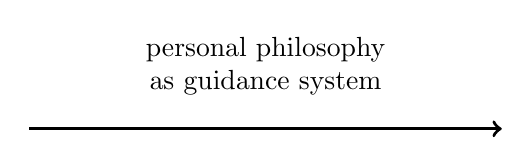
\begin{tikzpicture}[x=1cm,y=1cm]
\draw[->, very thick] (0,0) -- (6,0);
\node[align=center] at (3,0.8) {personal philosophy\\as guidance system};
\end{tikzpicture}
\caption{A cautious reconstruction of the lecture's first board idea: philosophy gives direction before it gives detail.}
\end{figure}

The lecture insists that the guidance system is not an ornament. It performs work. It must begin early, before temptation becomes habit and before carelessness becomes destiny. Parents, teachers, early ideas, and early information all belong to this first system because the whole later structure depends on it.

\subsection{Question \& Answer}

What does the guidance system actually do?

Rohn gives a precise answer. It does two things and only two things:
\begin{equation}
G \longrightarrow \{\text{danger},\ \text{opportunity}\},
\end{equation}
where \(G\) denotes the guidance system.

First, it helps us see dangers early enough not to build on sand simply because the sky is blue and the clouds are soft. Second, it helps us find opportunities clearly enough not to drift past them by accident. The striking feature here is that both functions are needed at once. A life can be ruined by attraction to the wrong thing just as easily as it can be impoverished by blindness to the right thing.

\section{High Drama: Opposites, Temptation, and Conflict}

Once the guidance system is drawn, the lecture immediately places it in a world where it is needed. This world is not flat. It is dramatic. Danger and opportunity ride side by side. That is the phrase, and it governs everything that follows.

The Los Angeles traffic example is not merely comic. It is an exact miniature of the general structure. A green light does not abolish danger. If one walks or drives with naive literalism, one may be destroyed by the car that is still running the red. The point is then widened through the cartoon of angel and devil whispering from opposite shoulders, and widened again through the image of the decent man who is late, runs the light, and dies. The lecture is careful: this is not an evil man, not a monstrous man, but a careless man. A moment of thoughtlessness is enough.

The paired structure of the lecture can be compressed into a narrow table:
\begin{table}[h]
\centering
\begin{tabular}{p{0.34\linewidth} p{0.34\linewidth}}
danger & opportunity \\
evil & good \\
darkness & light \\
illness & health \\
death & life \\
tyranny & liberty
\end{tabular}
\caption{The lecture's paired opposites. The list is not decorative; it is the working architecture of ``high drama.''}
\end{table}

Rohn's own compression of the whole section is worth preserving as a displayed formula:
\begin{equation}
\text{Opposites are in conflict and we are in the middle.}
\end{equation}

The biological metaphor makes the same point in another register. Red corpuscles nourish, white corpuscles fight. Friendly bacteria and unfriendly bacteria coexist. The war is already running. The lecture is not doing biology for its own sake. It is insisting that conflict is structural, not accidental.

\subsection{Question \& Answer}

Why must danger and opportunity remain side by side?

Because otherwise the language of victory would become empty. The lecture answers this several ways. A book in which every chapter says that everything is fine is a dead book. A football crossed over the line without defenders is not a touchdown. Winning requires the possibility of losing. Contest gives meaning to achievement. Thus we may write the stripped-down lecture logic as
\begin{equation}
\text{no possibility of loss} \quad \Rightarrow \quad \text{no meaningful win}.
\end{equation}
Danger is therefore not introduced to glorify danger. It is introduced to explain why judgment matters, why vigilance matters, and why the guidance system must remain active.

\section{Wind, Sail, and the Five-Year Redesign}

At the very point where ``high drama'' might tempt us into fatalism, the lecture turns sharply toward agency. It does so with the sailboat analogy. The winds are always blowing: contrary winds, political winds, social winds, familiar winds, unfamiliar winds, and the severe winds of storm. But to get where we want to go, Rohn says, we do not have to curse the wind. We have to set a better sail.

A compact editorial rendering of the argument is
\begin{equation}
\text{destination}=f(W,S),
\end{equation}
where \(W\) stands for winds or external conditions, and \(S\) stands for the set of the sail.

\begin{remark}
This formula is a cautious reconstruction. The spoken claim is simpler and stronger: the wind will blow; the decisive human task is to improve the sail.
\end{remark}

The lecture even names some of the instruments by which a sail is improved: sermons, song lyrics, conversations with friends, and classes like the one being given. These are not ornamental supplements. They are sail-adjustment mechanisms. The point is not merely to survive future years, but to become so good at setting sail that changing winds still move us toward destination rather than away from it.

The board evidence now becomes broader. The same flip-chart page has accumulated several conceptual beats, and the precise words are unreadable. But its larger geometry remains useful.

\begin{figure}[h]
\centering

\includegraphics[width=0.70\linewidth]{lecture_19_figure_03.png}
\caption{The accumulated flip-chart layout during the wind-and-storm discussion. What survives clearly is the structure: a central route, clustered regions, and a rising alternative path.}
\end{figure}

\begin{figure}[h]
\centering
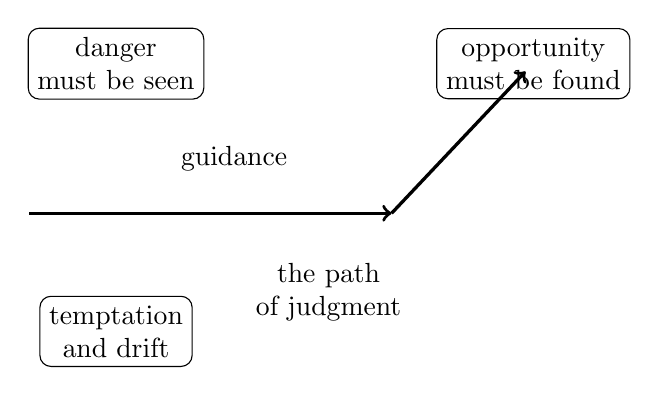
\begin{tikzpicture}[x=1cm,y=1cm]
\draw[->, very thick] (0.2,3.0) -- (4.8,3.0);
\draw[->, very thick] (4.8,3.0) -- (6.5,4.8);
\node[draw, rounded corners, align=center] at (1.3,4.9) {danger\\must be seen};
\node[draw, rounded corners, align=center] at (1.3,1.5) {temptation\\and drift};
\node[draw, rounded corners, align=center] at (6.6,4.9) {opportunity\\must be found};
\node[align=center] at (2.8,3.7) {guidance};
\node[align=center] at (4.0,2.0) {the path\\of judgment};
\end{tikzpicture}
\caption{A transcript-guided clarification of the board's logic: a central path, a dangerous side, and a rising opportunity side.}
\end{figure}

The sailboat metaphor then becomes human exceptionalism. A goose goes south because it is a goose. A tree cannot tear itself loose and relocate. But a human being can go north, south, east, or west by choice; can live one way for five years and another way for the next five; can tear up an old script and write a new one. This is where the lecture moves from navigation to redesign.

\subsection{Question \& Answer}

If the winds are given, what is actually ours to change?

The lecture's answer is concrete: not the wind, but the sail; not the past weather, but the present correction; not the mere fact of motion, but the direction of motion. The ``you are here'' moment on the board captures this answer in miniature.

\begin{figure}[h]
\centering

\includegraphics[width=0.70\linewidth]{lecture_19_figure_04.png}
\caption{Marking the current position on the five-year path sketch. The exact writing is uncertain, but the locator mark is the point.}
\end{figure}

We may summarize the redesign argument by distinguishing the present point \(x_0\), the destination reached by inertia, and the destination reached after correction:
\begin{align}
x_0 &\to x_{5,\mathrm{def}},\\
x_0 &\to x_{5,\mathrm{new}}.
\end{align}

\begin{figure}[h]
\centering
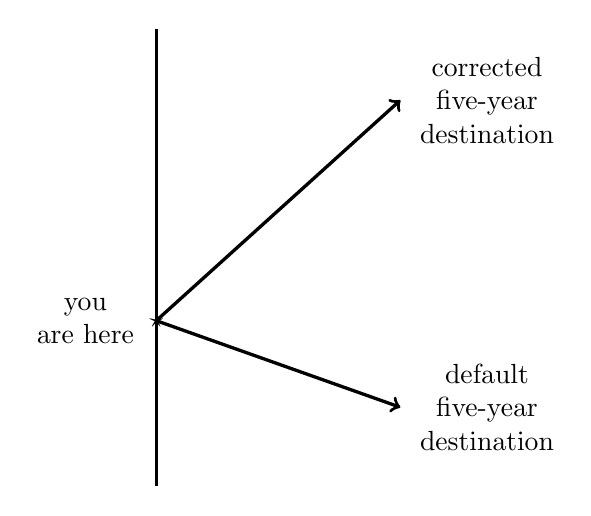
\begin{tikzpicture}[x=1cm,y=1cm]
\draw[very thick] (0,0) -- (0,5.8);
\draw[->, very thick] (0,2.1) -- (3.1,1.0);
\draw[->, very thick] (0,2.1) -- (3.1,4.9);
\node at (0,2.1) {$\star$};
\node[align=center] at (-0.9,2.1) {you\\are here};
\node[align=center] at (4.2,1.0) {default\\five-year\\destination};
\node[align=center] at (4.2,4.9) {corrected\\five-year\\destination};
\end{tikzpicture}
\caption{A narrow reconstruction of the redesign argument: continuation by inertia versus corrected direction.}
\end{figure}

\paragraph{Update rule.}
The logic of the redesign can be written as a worked sequence:
\begin{enumerate}
\item mark the present point \(x_0\);
\item extrapolate present daily activity to obtain \(x_{5,\mathrm{def}}\);
\item judge whether \(x_{5,\mathrm{def}}\) is acceptable;
\item identify errors in judgment, habit, and discipline;
\item correct the local direction of motion;
\item replace \(x_{5,\mathrm{def}}\) with \(x_{5,\mathrm{new}}\).
\end{enumerate}
This is exactly the simple analysis that Rohn attributes to his age-\(25\) turn: review the previous years, locate the errors, invest the corrections into the next years.

\section{Testimonials, Attitude, and Goal Formation}

After the redesign argument, the lecture pauses and consolidates. It is not enough to say that redesign is logically possible. Rohn wants the audience to feel that the evidence is already abundant. Hence the repeated phrase: from testimonials and personal experience, we have enough information to conclude that an extraordinary life can be designed and lived. Its internal form is evidentiary:
\begin{equation}
\text{testimonials}+\text{personal experience}
\Longrightarrow
\text{it is possible to design and live an extraordinary life}.
\end{equation}

The lecture then performs an important bridging move. Before introducing attitude, it briefly returns to the positive side of the earlier contrast structure. Personal philosophy is not merely about noticing darkness and danger. It is about cooperating with the positive side. The body calls for one thing and receives another; health works for us and asks whether we are on its side. The same structure is extended outward: more liberty than tyranny, more light than darkness, more health than illness, more opportunity than danger. These are, he says, extraordinary times. The consequence is motivational: if there was ever a time to put life systems in order and multiply them by \(2\), \(3\), \(5\), or \(10\), this is the time.

Only now does the lecture move to attitude proper. Rohn divides attitude into four directions. We need a right attitude toward the past, so that we use the past rather than live in it. We need a right attitude toward the future, so that we have inspiration. We need a right attitude toward everybody else, because leadership is impossible without appreciation of the many. And we need a right attitude toward ourselves, because self-esteem creates self-confidence.

The transition from inspiration to method occurs through goals. We are told to decide what we want and write it all down: people to meet, books to read, classes to take, skills to learn, cities to visit, investments to have. Then comes the next key: begin checking them off. Put enough small things on the list to make checking immediate. If something large is checked off, celebrate it. The list grows by the energy released from completion.

\subsection{Question \& Answer}

How does inspiration become operational rather than merely emotional?

By attaching it to explicit objects that can be named, pursued, counted, and checked off. A goal is a future item made concrete enough to enter a list. A completed goal is not vague encouragement; it is a mark of actual motion. The lecture's psychological mechanism may be summarized as
\begin{equation}
\text{self-esteem} \to \text{self-confidence} \to \text{larger action}.
\end{equation}

Rohn then widens attitude toward others in a way that prepares the later lifestyle section. One person does not make an economy, an orchestra, or an enterprise. It takes everybody. The discussion of the gifts brought into America, the appreciation of music in Rome, and the reverence for excellence all belong here. Attitude is not merely inward mood. It is an educated relation to value outside oneself.

\section{Activity, Labor, and the Rejection of Empty Affirmation}

The lecture now turns from value and attitude to the third major idea: activity. This is where rhetoric becomes mechanism. Rohn calls work the miracle piece. Later he will even say that six-sevenths of life are spent in activity that creates career, relationship, city, future, wealth, power, and influence. The point is not exhaustion for its own sake. The point is transformation.

The old formula appears in plain form:
\begin{equation}
6\ \text{days labor} + 1\ \text{day rest}.
\end{equation}
In compact notation,
\begin{equation}
6:1.
\end{equation}
And the lecture adds the practical warning immediately: do not rest too long, or the weeds take the garden.

At this stage Rohn confronts a nearby counterfeit: affirmation without work. He does not deny that affirmation may have a place. He insists that it must be tied to truth. If one is broke, the truthful statement is the useful one. The diagnostic force lies in naming the condition honestly enough that change becomes necessary.

\subsection{Question \& Answer}

Why is affirmation alone not enough?

Because affirmation does not itself perform the transformation. Labor performs the transformation. The line the lecture wants us to keep is therefore
\begin{equation}
\text{affirmation without discipline} \to \text{delusion}.
\end{equation}

The deeper mechanism can be written in the paired form
\begin{align}
\text{wisdom}+\text{faith} &\not\Rightarrow \text{result}
\qquad \text{without activity},\\
(\text{wisdom}+\text{faith}) \xrightarrow{\text{activity}} \text{result}.
\end{align}
Rohn's list of results is concrete and social: cities, careers, fortunes, relationships, health, offices. Even the lecture itself is included under the same rule. He comes to do work of language and work of words. If those words land and are taken up by listeners, then the work propagates.

Thus ``miracle working days'' does not mean escape from labor. It means that labor is precisely the human share in turning nothing into something.

\section{Measurement, Lifestyle, and the Closing Spiral}

The next idea is measurement. Once work has been made central, the danger becomes delusion: we may imagine progress because something looks fine from a distance. The lecture answers with a counting discipline:
\begin{equation}
\text{progress}=\text{measurable in reasonable time}.
\end{equation}

Reasonable time is defined by exclusion. Five minutes is too short. Five years is too long. The daily horizon becomes the baseline. End of day: count, measure, look. Did the conversation happen? Was the anger settled? Was the health practice kept? Has the number changed?

\begin{table}[h]
\centering
\begin{tabular}{p{0.28\linewidth} p{0.46\linewidth}}
too soon & every five minutes \\
reasonable & by the end of the day \\
too late & after five years of not looking
\end{tabular}
\caption{The lecture's measurement cadence.}
\end{table}

The child-level model makes the point elegantly:
\begin{equation}
1\ \text{grade} / 1\ \text{year}.
\end{equation}
This is not because life is school. It is because the example makes progress countable. Property counts, income counts, health counts, and the building of a financial wall around one's family all inherit the same logic.

\subsection{Question \& Answer}

Why must we measure when things may already look fine from the outside?

Because appearance is not structure. The vineyard may look good while little foxes are already spoiling the vines. A bank account may be full while something quieter is going wrong. Therefore the lecture's practical theorem becomes
\begin{equation}
\text{success is a numbers game}.
\end{equation}
Count, check, and do not wait for government, society, or anyone else to build the measuring system for you.

At this point the lecture spirals outward again. The five ideas are recapped, and the long-standing Zig Ziglar debate between education and motivation is retold in miniature. Philosophy is education; attitude is motivation; both are needed. The hard work of learning and study is itself part of the same larger labor.

Then comes the final enlargement: lifestyle. The essence of life is not the Ferrari and not the bank account. A good life includes productivity, enduring friendship, heritage kept alive, spirituality studied and practiced and taught, and a refusal to miss the concert, the game, the class, the show, the conversation, the sermon. One hears in this last movement that the lecture has not abandoned business at all. It has instead inserted business into a larger theory of lived value.

The section on recognizing extraordinary value deepens this closing move. The cultivated bottle of wine, the poem, the song, the conversation, the photograph, the refined gesture: all are examples of a human faculty that can recognize what is fine. The point is not consumer luxury. The point is trained perception.

The final theological image completes rather than interrupts the chapter. If we plant the seed, the making of the tree belongs to a larger order than our immediate control. But we are invited to participate in the working of miracles. Hands, language, soul, compassion, enterprise, community: the lecture closes by placing all of them inside the dignity of work.

\section{Summary}

The chapter begins with a ladder and ends with a life. The ladder proves that large gains in earnings are possible. The lecture then shifts the operative variable from income itself to value brought to the marketplace, and from there to personal development. Philosophy becomes a guidance system, guidance is placed inside a world of opposed possibilities, and the world of opposites is then answered by the human power to set a better sail and redesign a five-year future. Testimonials stabilize this possibility, attitude gives it motive force, activity gives it causal power, and measurement gives it discipline. The closing theme of lifestyle then broadens the entire discussion: we are not only trying to earn more, but to live deliberately enough to recognize value, cooperate with the positive side, and participate in work that becomes larger than the self.